\documentclass{mcmthesis}
\mcmsetup{CTeX = false,    % 使用 CTeX 套装时,设置为 true
          tcn = {2520861}, problem = \textcolor{red}{C},
          sheet = true, titleinsheet = true, keywordsinsheet = true,
          titlepage = false, abstract = false}
        
\usepackage{newtxtext}     % \usepackage{palatino}
\usepackage[style=apa,backend=biber]{biblatex}
\addbibresource{reference.bib}

\usepackage{tocloft}
\usepackage{subcaption}
\usepackage{float}  %控制图片和表格的位置
\usepackage{indentfirst} %s首行缩进
\usepackage{threeparttable} %添加表格注释
\setlength{\cftbeforesecskip}{6pt}
%\setlength{\parindent}{2em} %全局首行缩进2字符
\renewcommand{\contentsname}{\hspace*{\fill}\Large\bfseries Contents \hspace*{\fill}}

\title{{\bf title}}
% \author{\small \href{http://www.latexstudio.net/}
%   {
\includegraphics[width=7cm]{mcmthesis-logo}}}
\date{\today}

\begin{document}
%%%%%%%%%%%%%%%%%%%%%%%%%%%%%%%%%%%%%%%摘要%%%%%%%%%%%%%%%%%%%%%%%%%%%%%%%%%%%%%%%%
\begin{abstract}

    abstract content...

\begin{keywords}
    Momentum Analysis; Predictive Modeling; Random Forest; Sliding Window; Logistic Regression;
    Data Visualization; Generalization Capability
\end{keywords}
\end{abstract}


%%%%%%%%%%%%%%%%%%%%%%%%%%%%%%%%%%%%%%%目录%%%%%%%%%%%%%%%%%%%%%%%%%%%%%%%%%%%%%%%%
\maketitle

\tableofcontents
\thispagestyle{empty}

\newpage
%%%%%%%%%%%%%%%%%%%%%%%%%%%%%%%%%%%%%%%引言%%%%%%%%%%%%%%%%%%%%%%%%%%%%%%%%%%%%%%%%
\section{Introduction}

\subsection{Background}%%%%%%%%背景

\subsection{Literature Review}%%%%%%%%文献综述

\subsection{Restatement of the Problem}%%%%%%%%问题重述


\subsection{Our Work}%%%%%%%%文章分析


%%%%%%%%%%%%%%%%%%%%%%%%%%%%%%%%%%%%%%%假设%%%%%%%%%%%%%%%%%%%%%%%%%%%%%%%%%%%%%%%%%%%
\section{Assumptions and Justification}

%%%%%%%%%%%%%%%%%%%%%%%%%%%%%%%%%%%%%%%符号说明%%%%%%%%%%%%%%%%%%%%%%%%%%%%%%%%%%%%%%%%
\section{Notations}

%%%%%%%%%%%%%%%%%%%%%%%%%%%%%%%%%%%%%%%数据处理%%%%%%%%%%%%%%%%%%%%%%%%%%%%%%%%%%%%%%%%





%%%%%%%%%%%%%%%%%%%%%%%%%%%%%%%%%%%%%%%模型结构%%%%%%%%%%%%%%%%%%%%%%%%%%%%%%%%%%%%%%%%

\section{TASK3:Random Forest-based prediction of first-time award-winning countries}

\subsection{Random Forest Model}
To identify the key factors influencing the transition in the number of medals won by a country, two steps are required:
\begin{itemize}
\item {\bf First,}a predictive model is developed to predict the turning point where the number of medals shifts from zero to one.        
\item {\bf Second,}infer key indicators based on the model results.
\end{itemize}

\subsection{Data Preparation and Preprocessing}

\subsubsection{Data Table Construction}
    Construct three data tables, participation\_by\_year\_country, participation\_by\_year\_country\_count, and sport\_count\_pivot, to record the number of participants of the country each year, the cumulative number of participations by year, and the number of events participated each year, respectively.

    To exclude countries that did not win any medals, entries from the participation\_by\_year\_country table corresponding to countries listed in the NOC column of the medal\_counts table were deleted.

    In the medals\_by\_year and medals\_by\_year\_gold datasets, the historical data for each country was traversed to determine the year in which they first won a medal. If all values in a column were zero, None was returned. The results were then stored in first\_medal\_filtered for preview. This dataset only contains countries whose first medal or gold medal year is greater than or equal to 1920.

\subsubsection{Dataset Creation}

{\bf First Iteration:}
    For each country's NOC, corresponding information was extracted from the participation\_by\_year\_country\_count, participation\_by\_year\_country, and sport\_count\_pivot data frames:
\begin{itemize}   
\item {\bf participation\_count:} The number of times the country participated in the year it first won a medal.
\item {\bf events\_participation} The number of events the country participated in during the year it first won a medal.
\item {\bf sport\_count: }The number of sports the country participated in during the year it first won a medal.
These extracted values were then added to , which will serve as the basis for subsequent datasets.
\end{itemize}

These extracted values were then added to new\_table\_data, which will serve as the basis for subsequent datasets.

{\bf Second Iteration:}
    To obtain data from the four years prior to the first medal year, the data from the four years after the first medal year were subtracted.

{\bf Third Iteration:}
    For each country that had never won a medal, the country's NOC, participation\_count, events\_participation, and sport\_count were added to new\_table\_data as a list.

    Finally, the entire list of data stored in new\_table\_data was converted into a Pandas DataFrame. After filling in missing values and cleaning invalid data, the final dataset, tree\_dataset, was formed.

\subsection{ Model Construction}

\subsubsection{Variable Analysis}
After careful selection and consideration of the available limited data, we chose three feature variables to train the model. The detailed list of variables is as follows:

    \begin{table}[h] 
        \centering  
        \caption{Table of Variables}  
        \label{tab1} 
    \begin{tabular}{ll} 
        \toprule
        Indicator  & Descriptions \\    
        \midrule 
        $participation\_count$ & The number of participants from the country\\
        $events\_participation\_count$ & The number of times the country participated\\
        $sport\_count$   & The number of sports in which the country participated each time \\
        \bottomrule
    \end{tabular}
    \end{table}

    At the same time, our target variable is Will\_Earn\_Medal, which indicates whether a medal will be earned (1 or 0).

\subsubsection{Model Training}
   
    After standardizing the data using StandardScaler, the dataset was split into training and testing sets, with 80\% used for training and 20\% for testing.

    We utilized the aforementioned features as input parameters for the Random Forest model to train on the training set. The parameter grid for the Random Forest model was as follows:
    \begin{table}[h] 
        \centering  
        \caption{Input parameters for forest models}  
        \label{tab1} 
    \begin{tabular}{ccccc} 
        \toprule
        Indicator  & Descriptions \\    
        \midrule 
        $Number of Estimators$ & [50, 100, 150, 200]\\
        $Max Depth$ & [None, 10, 20, 30]\\
        $Min Samples Leaf$   & [2, 5, 10] \\
        $Min Samples Split$ & [1, 2, 4]\\
        $Max Features$ & ['auto', 'sqrt', 'log2']\\
        \bottomrule
    \end{tabular}
    \end{table}

    We employed the RandomForestRegressor algorithm from the scikit-learn (sklearn) machine learning library, along with the GridSearchCV method for hyperparameter tuning. The optimal hyperparameter combination obtained from GridSearchCV was as follows:

    \begin{table}[h] 
        \centering  
        \caption{Optimal hyperparameter combination}  
        \label{tab1} 
    \begin{tabular}{ccccc} 
        \toprule
        Indicator  & Descriptions \\    
        \midrule 
        $Number of Estimators$ & 200\\
        $Max Depth$ & 10\\
        $Min Samples Leaf$   & 1 \\
        $Min Samples Split$ & 2\\
        $Max Features$ & sqrt\\
        \bottomrule
    \end{tabular}
    \end{table}

\subsubsection{Model Performance Visualization}

    To assess the performance of the mod

\begin{itemize}   
    \item {\bf Confusion Matrix} :Displays the relationship between the model's predictions and the true labels, helping to analyze the types of errors made by the model.
    \item {\bf ROC Curve}: Plots the Receiver Operating Characteristic (ROC) curve, which measures the model's performance across different thresholds.
\end{itemize} 

    The confusion matrix and ROC curve are shown below:

\begin{figure}[H]
    \centering
    \begin{subfigure}{0.4\textwidth}
        \centering
        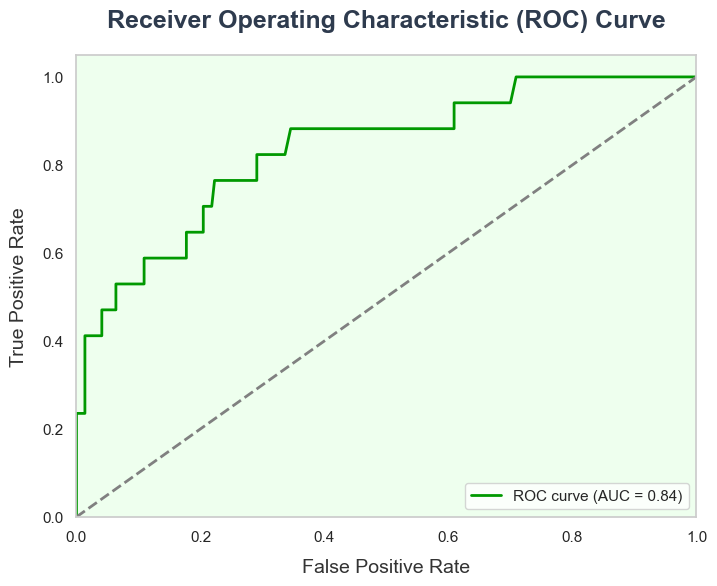
\includegraphics[width=\textwidth]{graph/rf_roc.png}
        \caption{ROC Curve}
        \label{subfig:player1}
    \end{subfigure}
    \hfill
    \begin{subfigure}{0.4\textwidth}
        \centering
        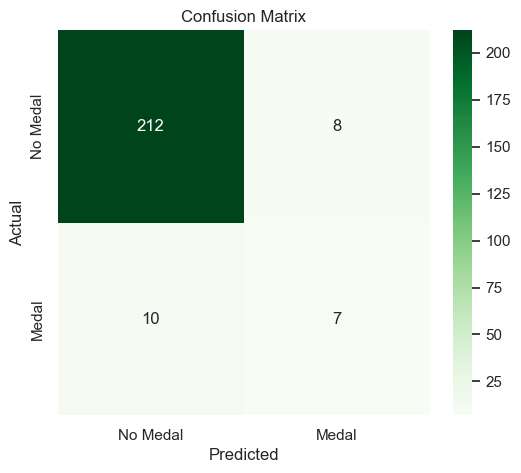
\includegraphics[width=\textwidth]{/graph/rf_confusion_matrix.png}
        \caption{Confusion Matrix}
        \label{subfig:player2}
    \end{subfigure}
    \caption{Model Performance Visualization}
    \label{Figure 13}
\end{figure}

    The confusion matrix indicates that the model's prediction accuracy is 94\%, with a false positive rate of only 0.039 (9/233), suggesting that the model is highly reliable and that most samples are correctly classified. The match between the predicted values and the true labels in the test set is high.

    The model's AUC (Area Under the Curve) is 0.87, demonstrating strong discriminative power and the ability to effectively distinguish between positive and negative classes. Additionally, the ROC curve rapidly rises in the low false positive rate (FPR) region, indicating that the model achieves a high recall rate while maintaining a low false positive rate. The model's true positive rate is commendable.

\subsubsection{Model Prediction}
    Using the best-trained model, {\bf best\_rf\_model}, we predicted the outcomes for new standardized data. The predict\_proba() method returns the probability of each sample belonging to each class, which allows us to calculate the probability of each country winning a medal.

\subsection{Model Testing}

\subsubsection{Test Set Construction}

    To validate the model's performance in real-world prediction tasks, we identified and selected historical samples of countries that have never won a medal from the {\bf athletes} dataset. We used a temporal grouping method to ensure the continuity and completeness of the data. After standardizing the feature data and applying quality control measures, we ultimately formed a high-quality test dataset.

    A new dataset containing relevant statistical data for all countries that have never won a medal was generated for the year 2024.

\subsubsection{Testing}

    Using the trained Random Forest model {\bf best\_rf\_model}, we predicted the features for each country and calculated the probability of each country winning a medal. These probabilities were stored in a list, sorted, and the countries most likely to win a medal were identified. A bar chart was then generated to visualize the predicted probabilities of each country winning a medal.

    Through probability distribution analysis, it was found that the prediction results exhibit distinct layering. Countries with a predicted probability greater than 0.20 are primarily concentrated in emerging market nations with well-developed sports infrastructure. These countries generally show consistent investment in sports and the specialization of sports programs.

\begin{figure}[h]   
    \centering          
    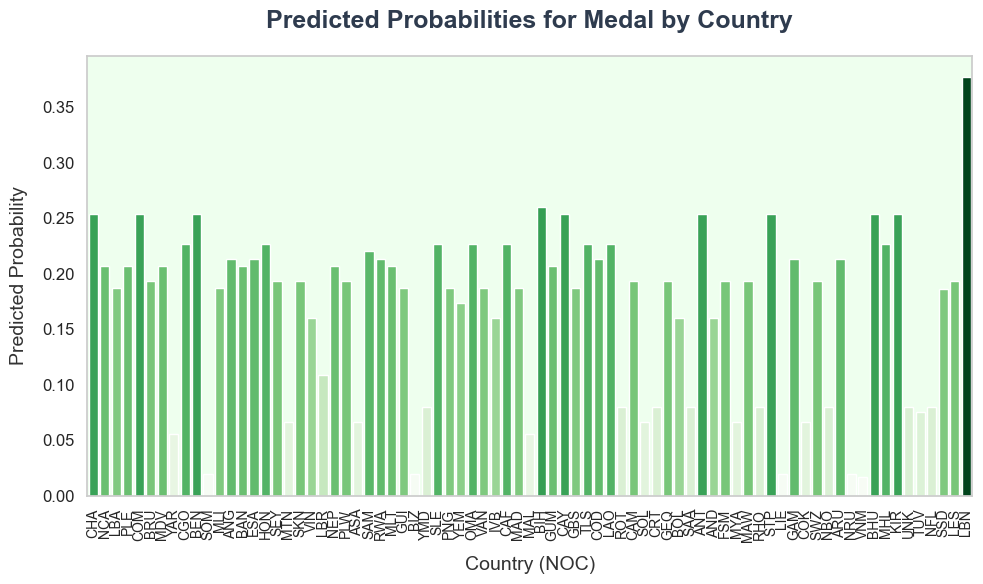
\includegraphics[width=12cm]{graph/rf_prediction.png}
    \caption{baseline of graphy} \label{fig1}    
\end{figure}

%%%%%%%%%%%%%%%%%%%%%%%%%%%%%%%%%%%%%%%敏感性分析%%%%%%%%%%%%%%%%%%%%%%%%%%%%%%%%%%%%%%%%
\subsection{TASK4: Quantitative Graph Theory Model of the "Great Coach Effect" Based on Network Flow}

\subsubsection{Model Background}

\subsubsection{Model Construction}

%\subsubsubsection{Construction of the Basic Directed Graph}

\begin{figure}[H]
    \centering
    \begin{subfigure}{0.45\textwidth}
        \centering
        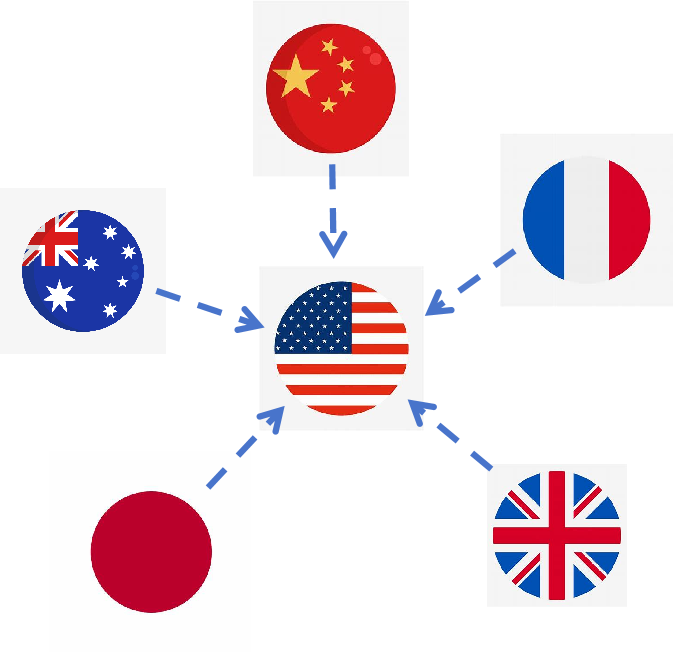
\includegraphics[width=\textwidth]{graph/graphy super country.png}
        \caption{super country type}
        \label{subfig:player1}
    \end{subfigure}
    \hfill
    \begin{subfigure}{0.45\textwidth}
        \centering
        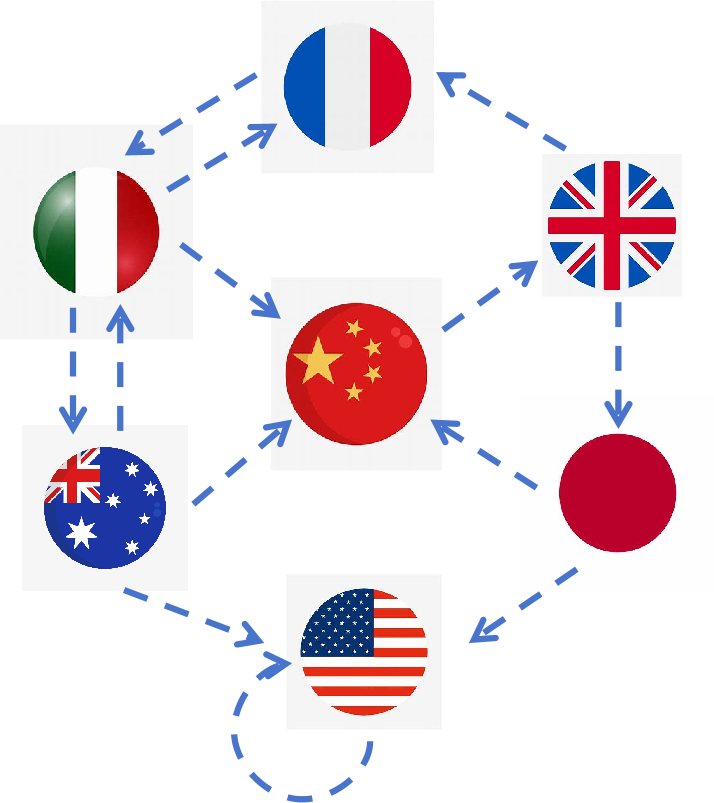
\includegraphics[width=\textwidth]{graph/graphy country flow.png}
        \caption{Large country circulation type}
        \label{subfig:player2}
    \end{subfigure}
    \caption{graph theory model}
    \label{Figure 13}
\end{figure}

%%%%%%%%%%%%%%%%%%%%%%%%%%%%%%%%%%%%%%%敏感性分析%%%%%%%%%%%%%%%%%%%%%%%%%%%%%%%%%%%%%%%%
\subsection{Letter}

Dear Sir or Madam

It is a great honour to write to you and share with you the results of our analysis of Olympic medal predictions. As a global platform for competition, the Olympic Games not only showcase the pinnacle of athletic excellence, but also foster international unity. In our mathematical modelling of Olympic medal predictions, we have identified several key findings, including trends in gender participation, the impact of host nations on medal counts, and the potential of under-researched sports.

These insights not only reflect historical and current trends but also provide actionable strategic recommendations for National Olympic Committees in their preparations for future Olympic events. 

Here are the detailed analyses of these findings and the implications for future planning:

1.Through statistical analysis of Olympic participation data, it was found that gender participation has shown significant evolutionary characteristics. In the early Olympic Games, male athletes dominated (accounting for approximately 70\%), while in recent years, this proportion has gradually approached balance.

\begin{figure}[H]
    \centering
    \begin{subfigure}{0.45\textwidth}
        \centering
        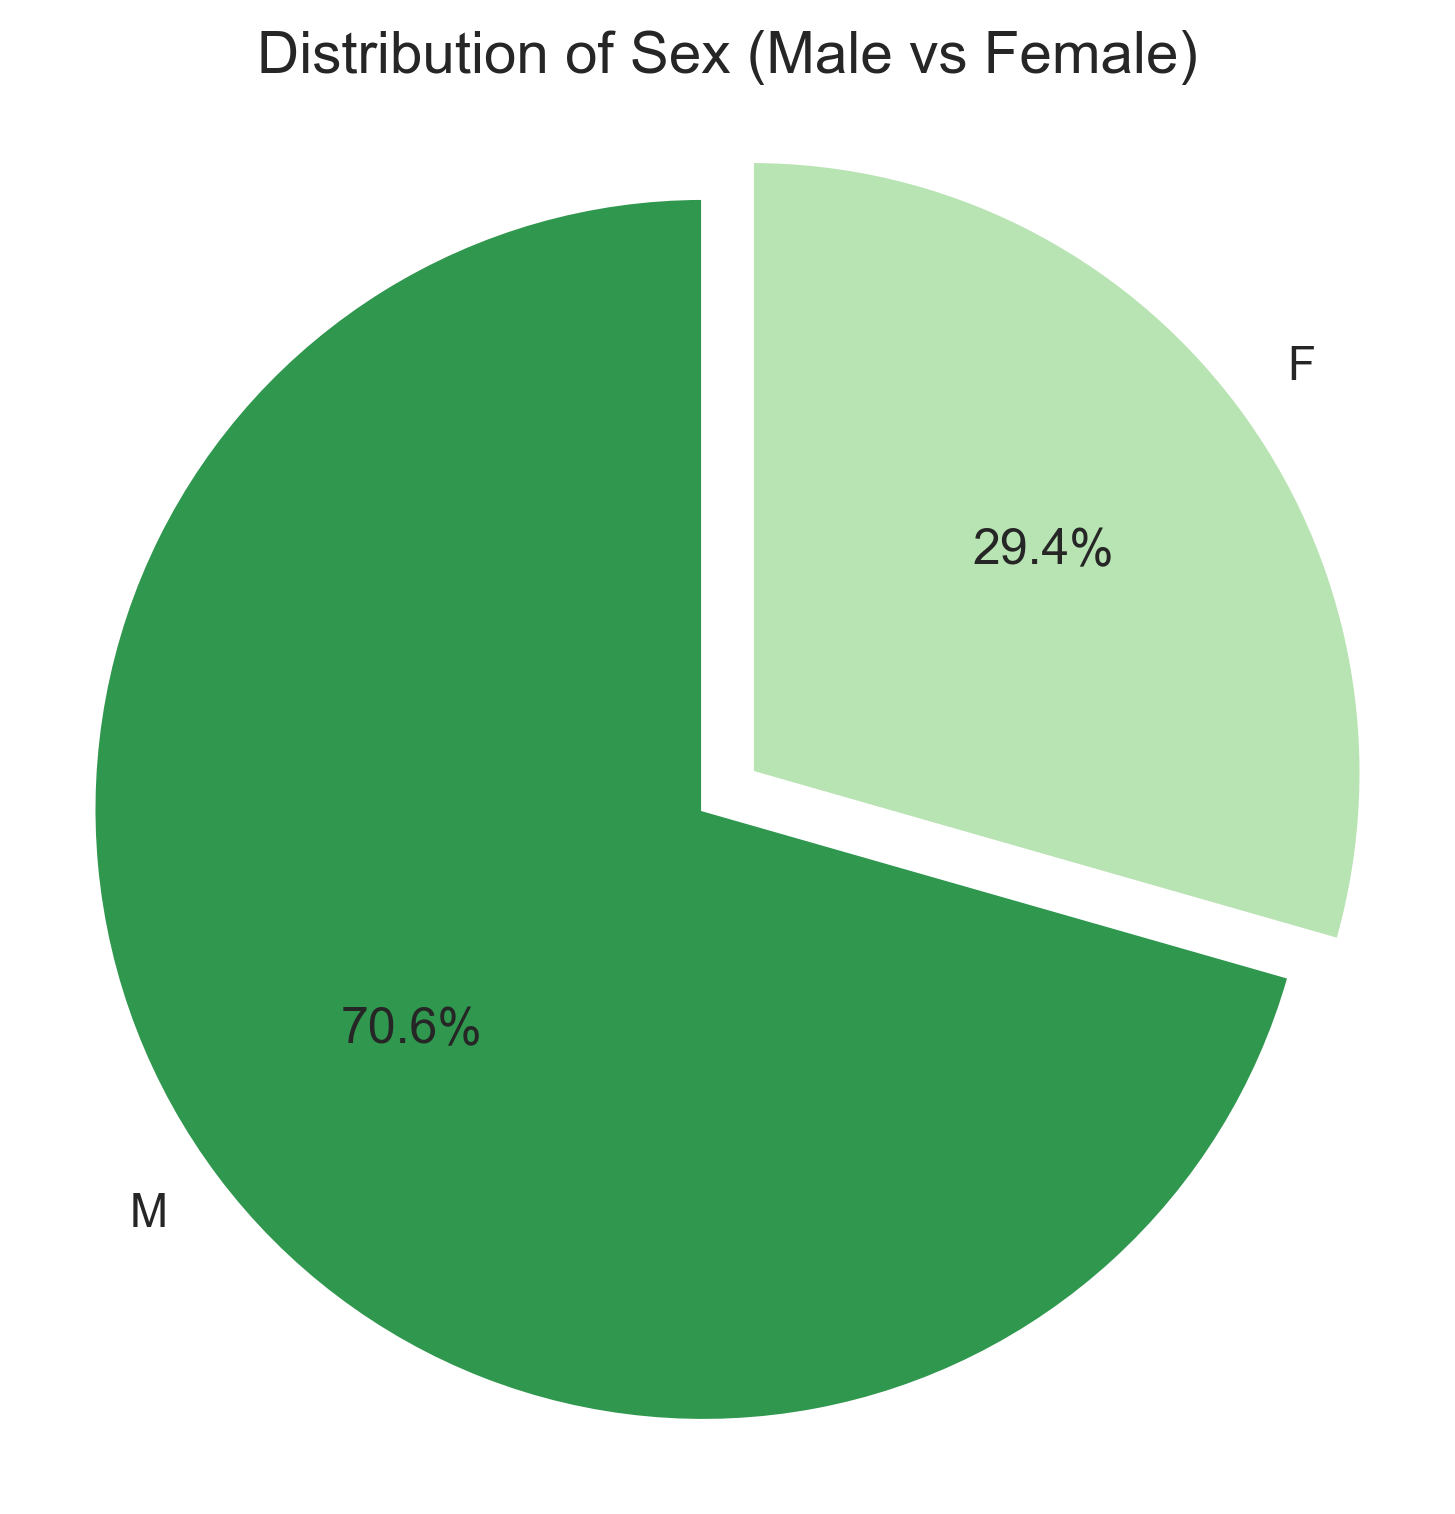
\includegraphics[width=\textwidth]{graph/Distribution of Sex.png}
        \caption{Distribution of Sex}
        \label{subfig:player1}
    \end{subfigure}
    \hfill
    \begin{subfigure}{0.45\textwidth}
        \centering
        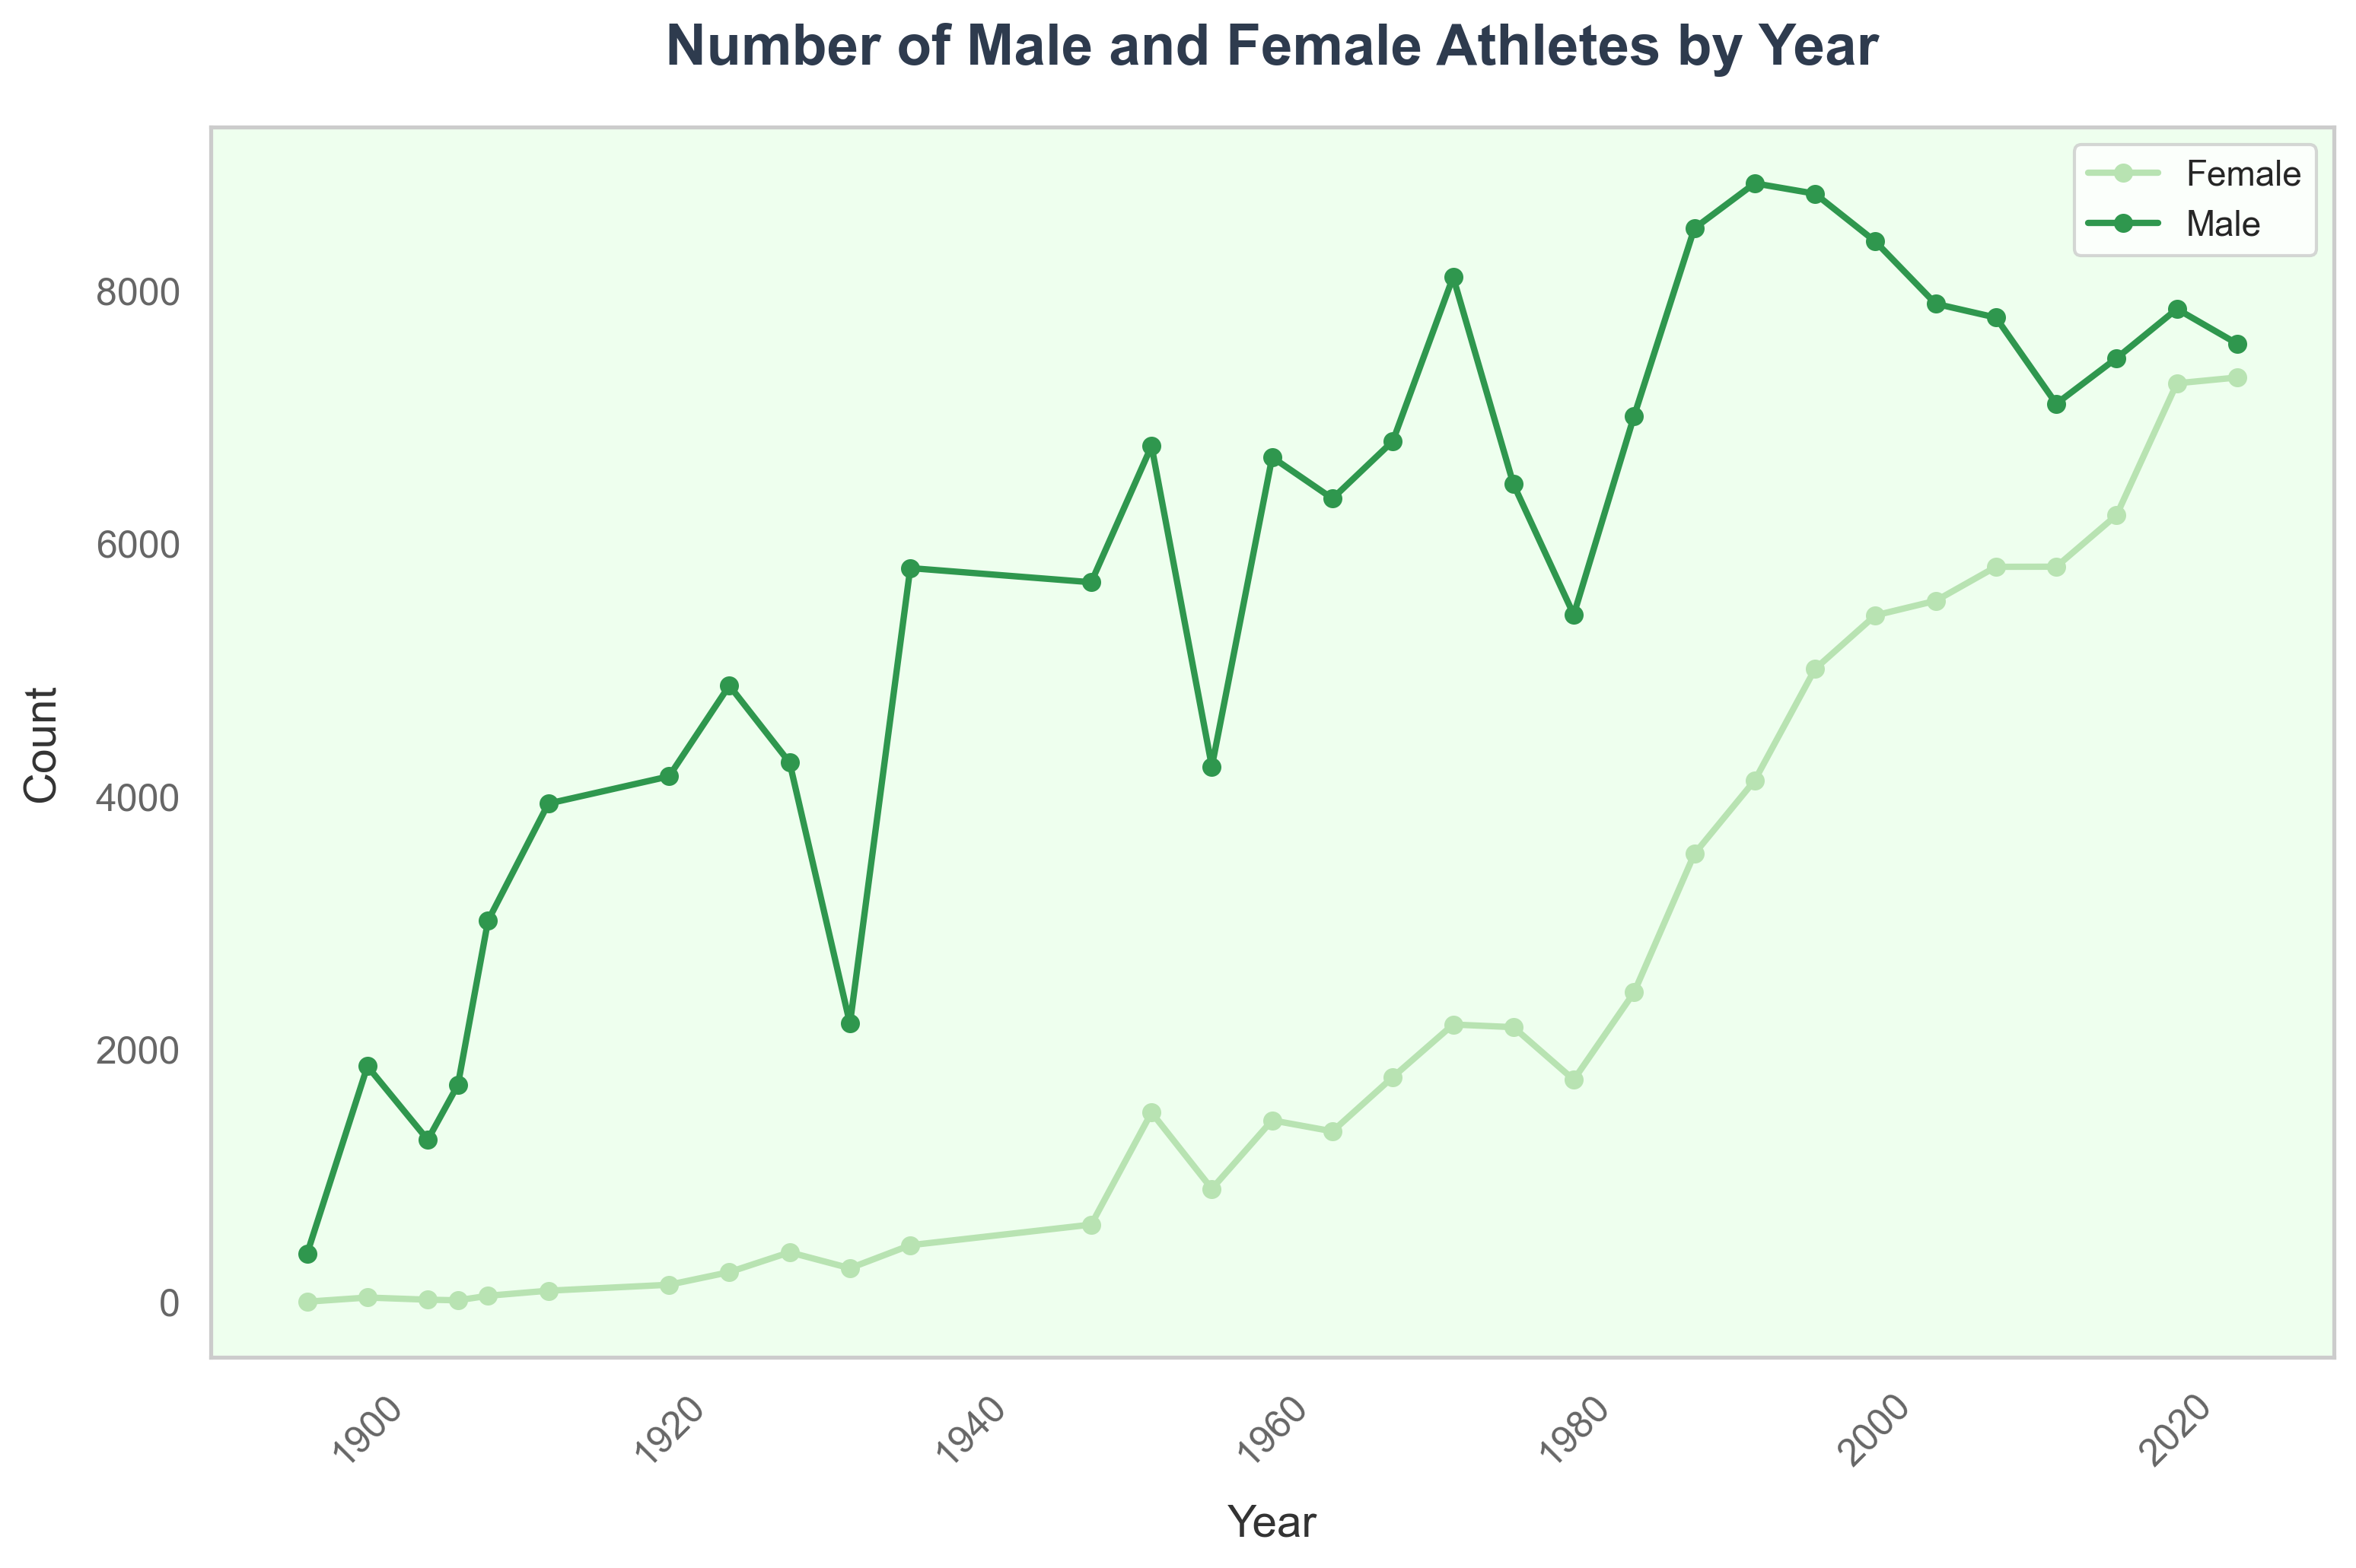
\includegraphics[width=\textwidth]{graph/Number_of_Athletes_by_Sex.png}
        \caption{Number of Male and Female Athletes by Year}
        \label{subfig:player2}
    \end{subfigure}
    \label{Figure 13}
\end{figure}

As seen in the chart above, after the 2012 London Olympics, the male-to-female athlete ratio came close to 1:1 for the first time, reflecting significant progress in gender equality at the Olympics. This phenomenon offers insights for improving performance in various countries:

\begin{itemize}   
    \item  National Olympic Committees (NOCs) can improve performance by increasing gender-equal events: As the participation of female athletes in the Olympics gradually increases, more mixed-gender events and 1:1 gender-equal competitions have emerged. Some countries can enhance their overall medal haul by promoting gender-equal participation.
    \item Gender differences in event settings impact total medal count: Some women's events, which were established later in Olympic history, have seen an increase in participation in recent years. However, when considering the number of sub-events, women's events are still relatively disadvantaged. This gender imbalance in event settings may affect certain countries' medal performance in specialized events. NOCs should pay attention to adjusting their preparation strategies to maximize their advantages in different gender-specific events.
\end{itemize}  

    2.When observing the annual medal counts of each country, we found that being the host nation had a significant impact on the increase in medal counts. As a result, we used the least squares method to verify the impact of hosting the Olympics on a country's medal count. This influence mainly comes from factors such as athlete fatigue from travel, familiarity with the venue, and the influence of home crowds on athletes. Therefore, host countries can improve their medal counts in the following ways:

\begin{itemize}   
    \item  Develop more detailed preparation plans based on historical experience and home advantage: Host countries can collaborate with their NOCs to add strength to their country's advantage in specific events and reduce weaker areas to boost their medal count. For instance, the US Olympic Committee has added five new sports for the 2028 Olympic Games in Los Angeles:  Baseball/Softball, Flag Football, Cricket (Twenty20), Lacrosse (Sixes), and Squash. While baseball/softball enjoys global popularity, it is the "national sport" of the U.S., with a wide base of participation and spectatorship domestically. Similarly, flag football, which is much less popular worldwide than sports like weightlifting, is a sport almost exclusively known in the U.S.
    \item Provide more support in infrastructure and financial resources: NOCs, taking advantage of their host status, can invest more resources in athletes’ economic welfare and competition adaptability prior to the games. Additionally, athletes from host nations receive heightened expectations from the public, and this “patriotic drive” can motivate athletes to perform at their best.
\end{itemize} 

    3.We conducted a statistical analysis of the medal shares for each country in various events and ranked the events by the highest share, in ascending order, to identify events that have not been monopolized, such as equestrian, sport climbing, and rowing. This result reveals that when medal distribution is more even across countries, it implies that more countries have the opportunity to compete for medals, providing valuable insights for countries of different types.

\begin{itemize}   
    \item Insights for Olympic Powerhouses: NOCs from powerhouse countries should deeply analyze these'non-monopolized' events in depth to assess whether they can increase investment in these areas, nurture a new generation of athletes, and enhance performance in these events at the Olympics.
    \item Insights for Emerging Sports Nations: For emerging sports nations, the dominance of Olympic powerhouses in traditional major events such as athletics, swimming, and gymnastics is long-established. However, the "Great Coach" effect validated earlier provides new breakthroughs for these nations. For example, Kenya excels in long-distance running but lacks coaches; hiring a "great coach" could help break the long-standing monopoly of Olympic powerhouses. At the same time, this result provides a potential point for increasing medal counts: through precise event targeting and scientific training plans, emerging sports nations can quickly improve their competitiveness in 'non-monopolized' events and achieve remarkable results.
\end{itemize} 


\subsection{Model Assessment}

\subsubsection{Strengths}
\subsubsection{Weaknesses}

\end{document}